\section{Question I: Revisiting HW4 Bank Classification with New Tools (for dataset A)}
\subsection{Data preprocessing}
For this part of the assignment, the dataset had to be analyzed first as part of the preprocessing step to get the structure ,detect issues such as missing values and outliers. The bank marketing data(bank-additional.csv) has 4119 observations and 21 features.There was found to be 1230 unknowns in the categorical features of the dataset. Features that had unknowns were checked and there was found to be six features(job,marital,education,default,housing,loan) with unknowns( 0.96 ,0.3 ,4.1,  19.5, 2.6)\% respectively.Removing rows with missing values can be too limiting on some predictive modeling problems.The proportion of the unknown's is sparse , the mode of the categorical features was used to replace the unknown's. Also , the "duration" feature was dropped since this attribute highly affects the output target (e.g., if duration=0 then y='no').
The categorical predictor variables  were converted  to numerical using git dummies ,appending the structure to 47 features (4119,47).
Outliers were found by first finding the standard deviation of each feature and then using each standard deviation to find values in that specific feature that vary by more than 3 standard deviations. 

\subsection{Dividing data into training and testing}
 

\subsection{Applying classification}
%Figure~\ref{fig:fig1} shows the comparison between histogram plots of feature 9 and 24 before and after normalization. 


Neural Network (NN): The neural network has three main layers: input, hidden, and output layers. The input layer is equal to the number of features in the training data (52 features). The output layer has a single node (outputs either 1 or 0). There is two main decisions to be made when tuning a neural network: first


% \begin{itemize}
% \item min/max has range from 0 to 1
% \item z-score is centered around mean = 0 and is ideal for PCA
% \item all histograms have the same shape after cleaning
% \item feat 24 seems to look normally distributed, feat 9 is not
% \end{itemize}


%%%%%%%%%%%%%%%%%%%%%%%%%%%%%%%%%%%%%%%%%%%%%%%%%%%%%%%%%%%%%%%%%%%
%
% Commands to include a figure:
%
%%%%%%%%%%%%%%%%%%%%%%%%%%%%%%%%%%%%%%%%%%%%%%%%%%%%%%%%%%%%%%%%%%%

\begin{figure}[!ht]
 \centering
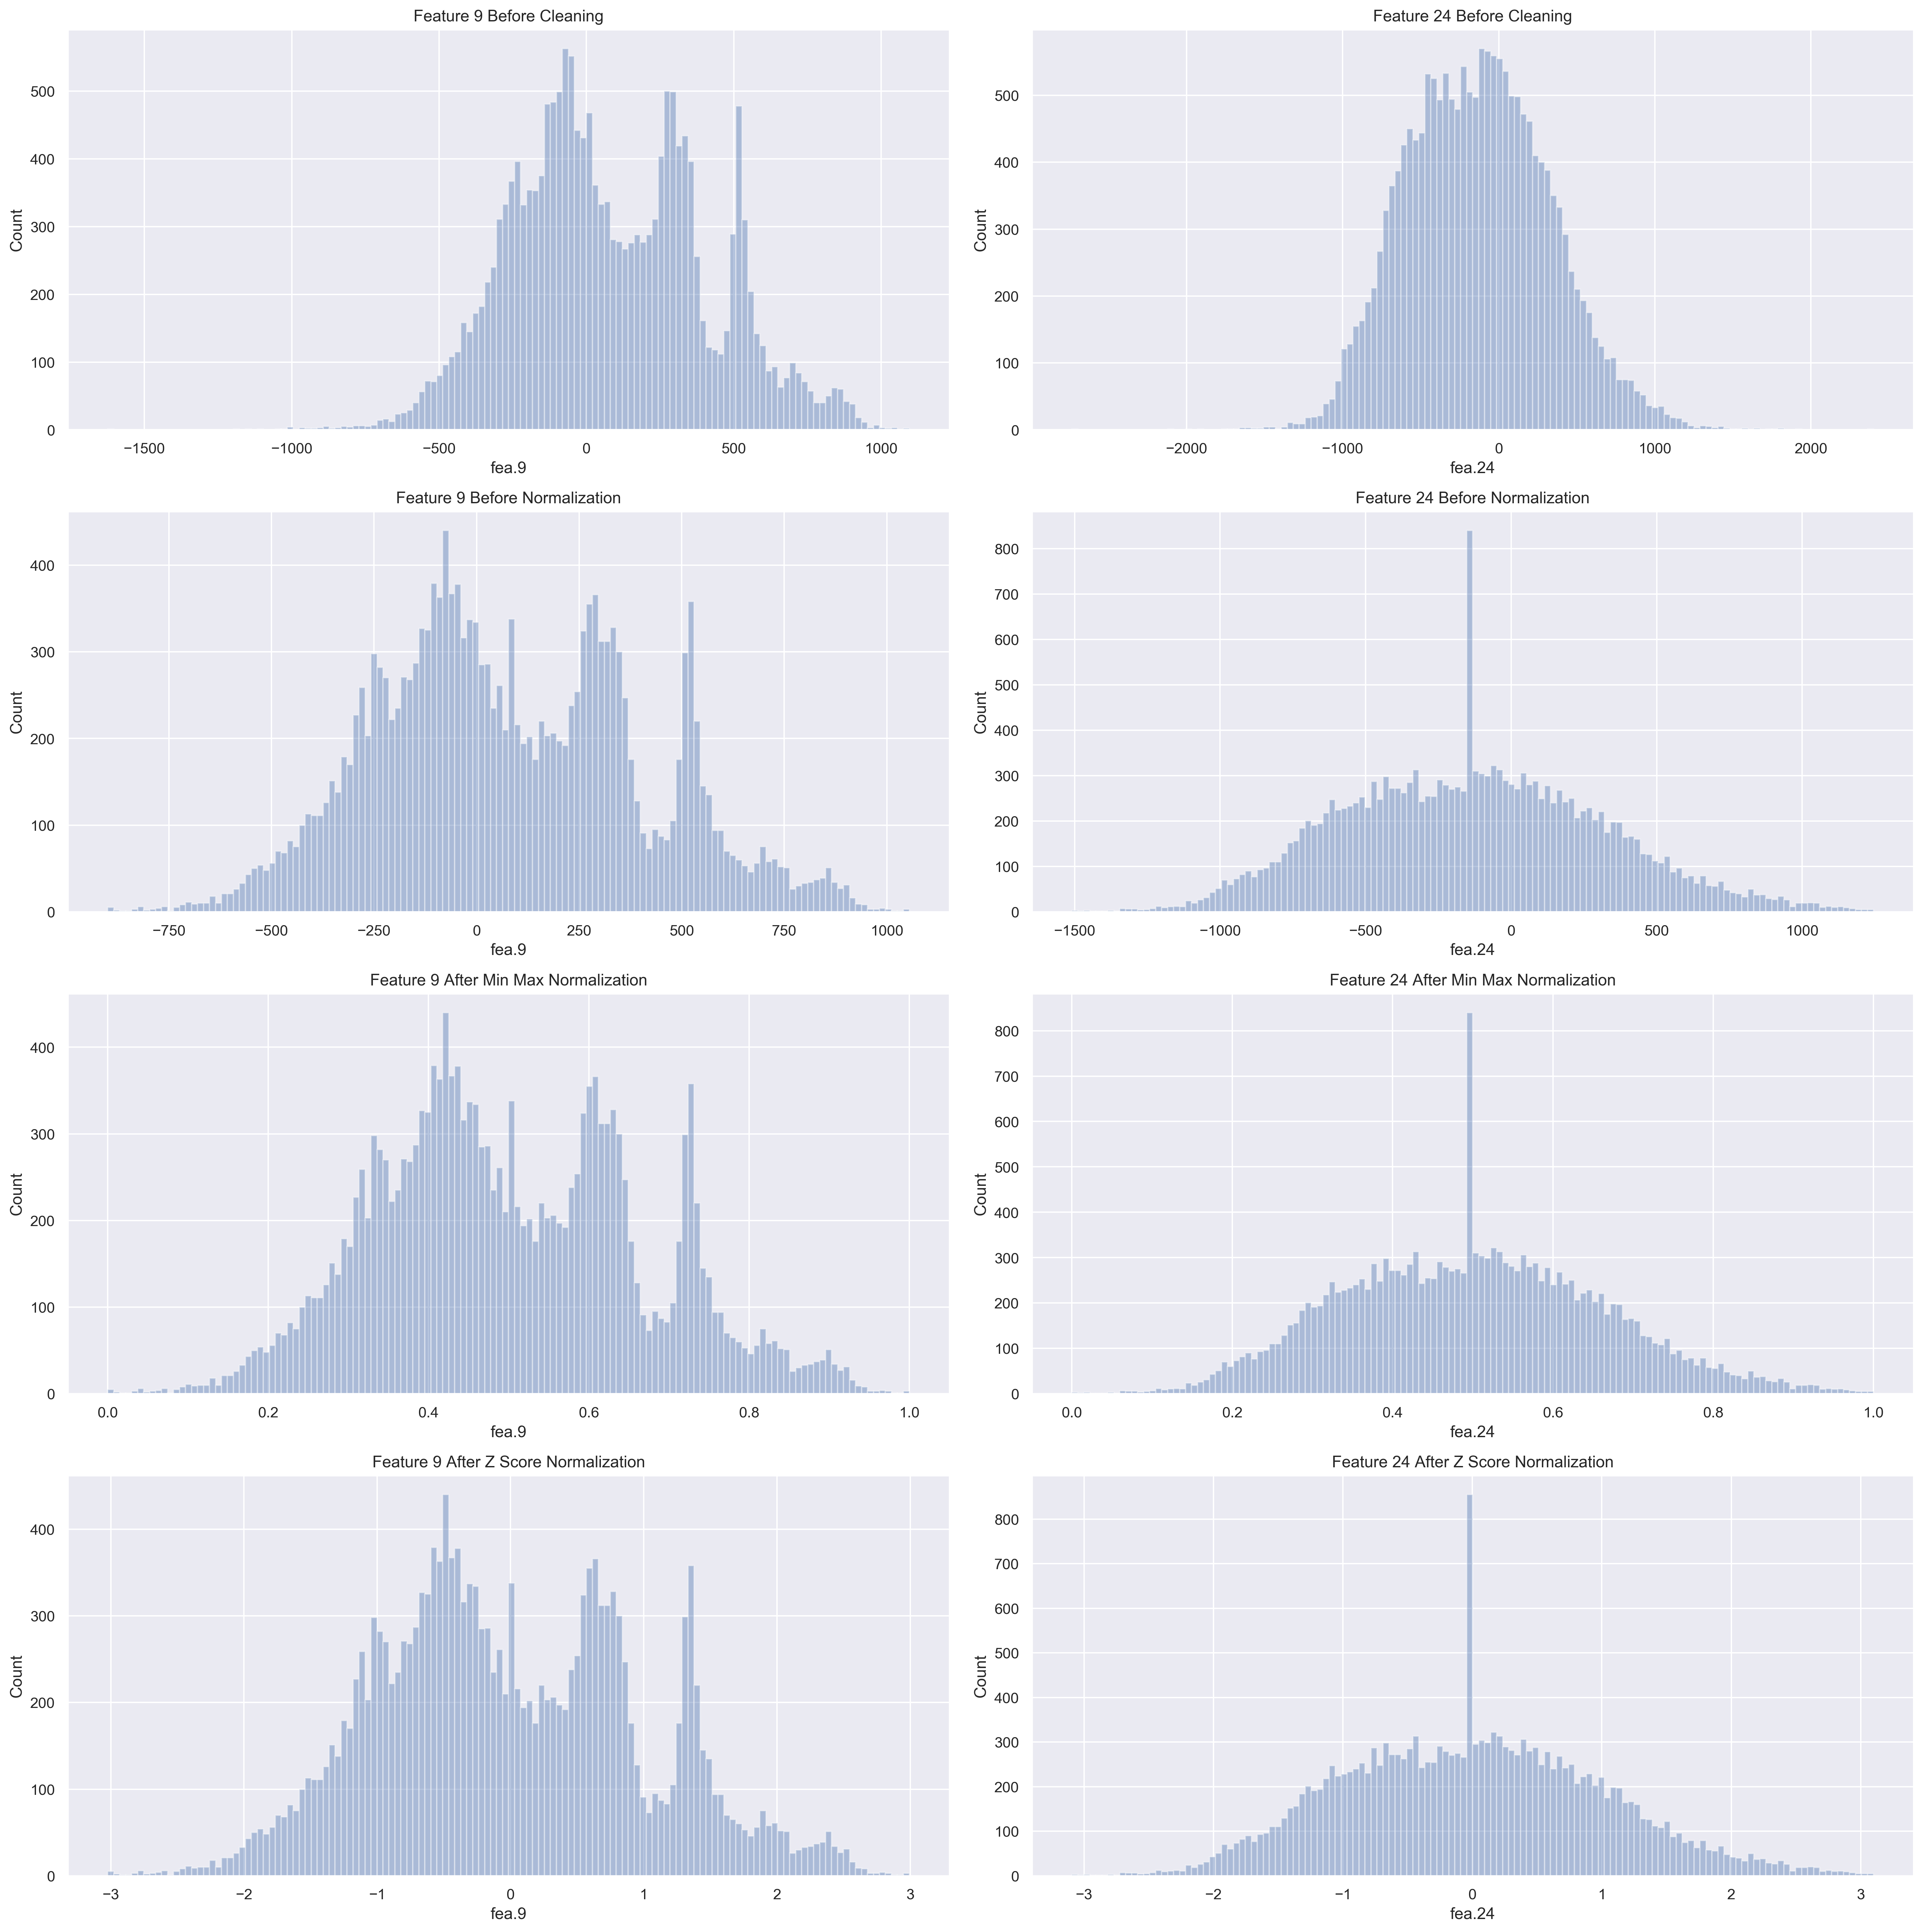
\includegraphics[width=6.1in]{assignment1/1-3-histograms.png}
\caption{\label{fig:fig1}histogram plots of feature 9 and 24 before and after normalization}
\end{figure}
